\documentclass[border=4pt]{standalone}
\usepackage{tikz}
\usetikzlibrary{shapes.symbols,positioning,arrows.meta}

\begin{document}
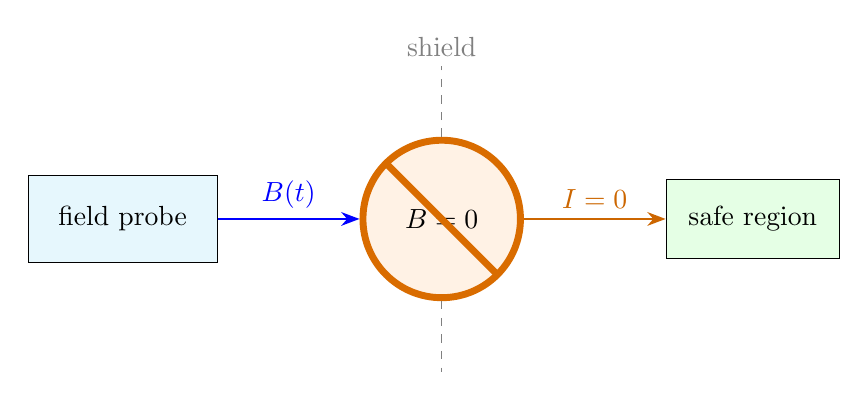
\begin{tikzpicture}[
  >=Stealth,
  node distance=18mm,
  detector/.style={draw,minimum width=24mm,minimum height=11mm,fill=cyan!10},
  exclusion/.style={correct forbidden sign,draw=orange!85!black,fill=orange!10,
    line width=2.5pt,minimum size=20mm,align=center}
]
  \node[detector] (sensor) {field probe};
  \node[exclusion,right=of sensor] (zero) {$B=0$};
  \node[draw,fill=green!10,minimum width=22mm,minimum height=10mm,
    right=of zero] (safe) {safe region};
  \draw[->,thick,blue] (sensor) -- node[above] {$B(t)$} (zero);
  \draw[->,thick,orange!80!black] (zero) -- node[above] {$I=0$} (safe);
  \draw[dashed,gray] (zero.north) -- ++(0,9mm) node[above] {shield};
  \draw[dashed,gray] (zero.south) -- ++(0,-9mm);
\end{tikzpicture}
\end{document}
